\documentclass[10 pt,usenames,dvipsnames, oneside]{article}
\usepackage{../../../modelo-ensino-medio}



\begin{document}

\begin{center}
  \begin{minipage}[l]{3cm}

\includegraphics[width=2cm]{logo}    
\end{minipage}\hfill
\begin{minipage}[r]{.8\textwidth}
 {\Large \scshape Atividade: Construindo uma Roda Gigante}  
\end{minipage}
\end{center}
\vspace{.2cm}

\ifdefined\prof
%Habilidades da BNCC
% \begin{objetivos}
% \item 
% \end{objetivos}

%Caixa do Para o Professor
\begin{goals}
%Objetivos específicos
\begin{enumerate}
\item Apresentar fenômenos periódicos por uma perspectiva
empírica
\item Construir gráfico de fenômeno que pode ser modelado por
função periódica
\item Identificar alguns elementos das funções periódicas
\end{enumerate}

\tcblower

%Orientações e sugestões
\begin{itemize}
\item Nesta atividade, além de apresentar um novo exemplo de
fenômeno periódico, pretende-se começar a explorar e
aprimorar conceitos associados a funções periódicas como
período e seus reflexos no gráfico da função (itens \titem{b)}, \titem{g)} e \titem{h)}), conjunto imagem, valor máximo e mínimo (itens \titem{d)} e
\titem{e)}) e o próprio formato não-retilíneo do gráfico da função
que modela esse exemplo (item \titem{f)}).
\end{itemize}
\end{goals}

\bigskip
\begin{center}
{\large \scshape Atividade}
\end{center}
\fi

Utilizando papelão, tampinhas de garrafa, cola e um lápis, construir uma roda gigante como a da figura.

\begin{figure}[H]
\centering

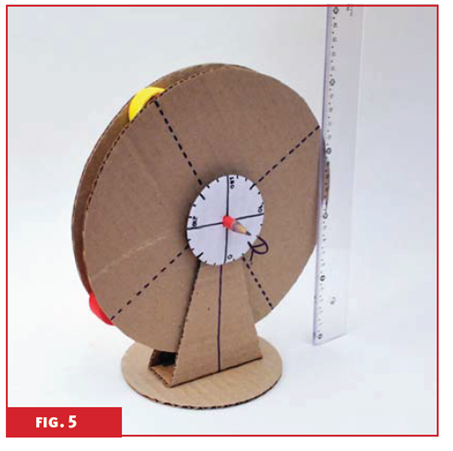
\includegraphics[width=.45\linewidth]{trigonometricas7}
\caption{Fonte: \cite{soares2010}}
\label{}
\end{figure}

Será necessário também o uso de um transferidor para medir os ângulos e uma régua para medir a altura das “cabines”.

Um passageiro entra na cabine quando essa está em seu ponto mais baixo. A partir daí, a roda começa a girar no sentido anti-horário, numa velocidade constante de $20$ graus por segundo. Considere $h = h(t)$ a altura em centímetros da cabine no instante de tempo $t$, medido em segundos.
\begin{enumerate}
\item Calcule a medida do raio da roda gigante e também as alturas mínima e máxima que a cabine pode assumir.
\item Quantos segundos a roda gigante demora para dar uma volta completa?
\item Com o auxílio dos seus colegas, encontre a altura da cabine em cada segundo do movimento da roda gigante até ela completar uma volta. Marque num papel milimetrado os pontos $(t,h(t))$ obtidos.
\item Entre a altura máxima e a altura mínima, há alguma altura intermediária que a cabine atinge mais de uma vez ao longo de cada volta da roda gigante? Quanto mede essa altura intermediária?
\item Determine todos os valores assumidos pela altura h da cabine ao longo de uma volta completa da roda gigante.
\item Observando os pontos marcados no item \titem{c)} e a dinâmica do giro da roda gigante, responda: apesar da velocidade com que a roda gigante gira ser constante, também será constante a taxa de variação da altura da cabine?  
\item Esboce no papel milimetrado uma curva que represente o gráfico de função $h = h(t)$. Como será o gráfico da função para valores de $t$ maiores que $18$ s?
\item Como seria o gráfico de $h = h(t)$ se a velocidade do giro da roda gigante duplicasse, ou seja, se ela demorasse apenas $9$ s para dar uma volta completa? Que alterações podem ser observadas em relação ao gráfico traçado no item \titem{g)}?
\end{enumerate}

\ifdefined\prof
\begin{solucao}

\begin{enumerate}
\item Isso irá depender da roda gigante construída para o
experimento.
\item $18$ segundos.
\item atividade prática.
\item Sim, todas as alturas intermediárias são atingidas 2 vezes
\item Isso dependerá da altura da roda gigante construída.
\item Não. Os instantes em que a cabine passa por pontos onde a
reta tangente à circunferência da roda gigante terão variação
da altura maior do que quando a cabine está no topo da roda
por exemplo.
\item Para $t>18$, o gráfico é a repetição
\item A função oscilaria mais rápido O gráfico ficaria mais
“comprimido”.
\end{enumerate}

\end{solucao}
\fi

\end{document}